\documentclass[12pt]{article}
\usepackage{tikz}
\usepackage{amsmath}
% Underlining package
\usepackage{ulem}
\usetikzlibrary{calc}
\usepackage[a4paper, portrait, margin=1cm]{geometry}
\usepackage{fancyhdr}

\def \HeadingQuestions {\section*{\Large Name: \underline{\hspace{8cm}} \hfill Date: \underline{\hspace{3cm}}} \vspace{-3mm}
{Angles in a Triangle: Questions} \vspace{1pt}\hrule}

% raise footer with page number; no header
\fancypagestyle{myfancypagestyle}{
  \fancyhf{}% clear all header and footer fields
  \renewcommand{\headrulewidth}{0pt} % no rule under header
  \fancyfoot[C] {\thepage} \setlength{\footskip}{14.5pt} % raise page number 6pt
}
\pagestyle{myfancypagestyle}  % apply myfancypagestyle

\newcounter{minipagecount}

\begin{document}
\HeadingQuestions
\vspace{8mm}

    \begin{minipage}{0.55\textwidth}
    \refstepcounter{minipagecount}
    \noindent{(\theminipagecount)}\quad
    \begin{tikzpicture}[scale=0.9, baseline=(current bounding box.north)]
        \begin{scope}[rotate=265]
            \coordinate (A) at (0,0);
            \coordinate (B) at (4.125,0);
            \coordinate (C) at (intersection cs: first line={(A)--($(A)+(75:4cm)$)}, second line={(B)--($(B)+(180-70:4cm)$)});
            \draw (A) -- (B) -- (C) -- cycle;

            % Mark angles with arcs;
            \draw ($(A)!0.3cm!(B)$) arc [start angle=0, end angle=75, radius=0.3cm];
            \draw ($(B)!0.3cm!(C)$) arc [start angle=180-70, end angle=180, radius=0.3cm];
            \draw ($(C)!0.3cm!(A)$) arc [start angle=180+75, end angle=360-70, radius=0.3cm];

            % Label angles
            \node at ($(A)!-0.25cm!(B)$) {G};
            \node at ($(B)!-0.25cm!(C)$) {F};
            \node at ($(C)!-0.25cm!(A)$) {H};

            % Mark angles in degrees
            \coordinate (midBC) at ($(B)!0.5!(C)$);
            \node at ($(A)!0.95cm!(midBC)$) {$75^\circ$};

            \coordinate (midAC) at ($(A)!0.5!(C)$);
            \node at ($(B)!0.95cm!(midAC)$) {$70^\circ$};

            \coordinate (midAB) at ($(A)!0.5!(B)$);
            \node at ($(C)!0.75cm!(midAB)$) {$\theta^\circ$};

          \end{scope}
        \end{tikzpicture}
    \end{minipage}%
    \hfill
    \begin{minipage}{0.4\textwidth}
        \begin{align*}
        \text{$\theta^\circ$} &= 180^\circ - (\angle \text{\dotuline{~~~~~~~}} + \angle \text{\dotuline{~~~~~~~}}) \\
        &= 180^\circ - (\dotuline{~~~~~~~}^\circ + \dotuline{~~~~~~~}^\circ) \\
        &= 180^\circ - \dotuline{~~~~~~~}^\circ \\
        &= \dotuline{~~~~~~~}^\circ
        \end{align*}
    \end{minipage}

\vspace{1cm} \vfill    \begin{minipage}{0.55\textwidth}
    \refstepcounter{minipagecount}
    \noindent{(\theminipagecount)}\quad
    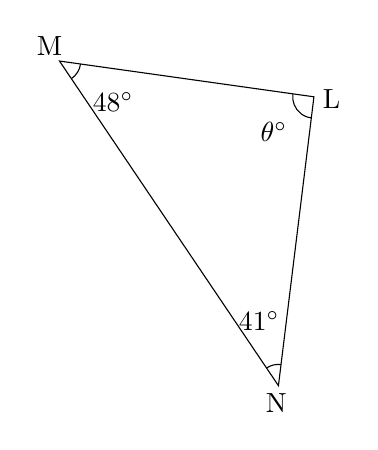
\begin{tikzpicture}[scale=0.9, baseline=(current bounding box.north)]
        \begin{scope}[rotate=304]
            \coordinate (A) at (0,0);
            \coordinate (B) at (5.525,0);
            \coordinate (C) at (intersection cs: first line={(A)--($(A)+(48:4cm)$)}, second line={(B)--($(B)+(180-41:4cm)$)});
            \draw (A) -- (B) -- (C) -- cycle;

            % Mark angles with arcs;
            \draw ($(A)!0.3cm!(B)$) arc [start angle=0, end angle=48, radius=0.3cm];
            \draw ($(B)!0.3cm!(C)$) arc [start angle=180-41, end angle=180, radius=0.3cm];
            \draw ($(C)!0.3cm!(A)$) arc [start angle=180+48, end angle=360-41, radius=0.3cm];

            % Label angles
            \node at ($(A)!-0.25cm!(B)$) {M};
            \node at ($(B)!-0.25cm!(C)$) {N};
            \node at ($(C)!-0.25cm!(A)$) {L};

            % Mark angles in degrees
            \coordinate (midBC) at ($(B)!0.5!(C)$);
            \node at ($(A)!0.95cm!(midBC)$) {$48^\circ$};

            \coordinate (midAC) at ($(A)!0.5!(C)$);
            \node at ($(B)!0.95cm!(midAC)$) {$41^\circ$};

            \coordinate (midAB) at ($(A)!0.5!(B)$);
            \node at ($(C)!0.75cm!(midAB)$) {$\theta^\circ$};

          \end{scope}
        \end{tikzpicture}
    \end{minipage}%
    \hfill
    \begin{minipage}{0.4\textwidth}
        \begin{align*}
        \text{$\theta^\circ$} &= 180^\circ - (\angle \text{\dotuline{~~~~~~~}} + \angle \text{\dotuline{~~~~~~~}}) \\
        &= 180^\circ - (\dotuline{~~~~~~~}^\circ + \dotuline{~~~~~~~}^\circ) \\
        &= 180^\circ - \dotuline{~~~~~~~}^\circ \\
        &= \dotuline{~~~~~~~}^\circ
        \end{align*}
    \end{minipage}

\vspace{1cm} \vfill    \begin{minipage}{0.55\textwidth}
    \refstepcounter{minipagecount}
    \noindent{(\theminipagecount)}\quad
    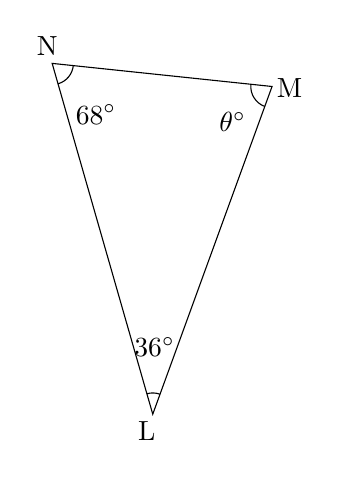
\begin{tikzpicture}[scale=0.9, baseline=(current bounding box.north)]
        \begin{scope}[rotate=286]
            \coordinate (A) at (0,0);
            \coordinate (B) at (5.15,0);
            \coordinate (C) at (intersection cs: first line={(A)--($(A)+(68:4cm)$)}, second line={(B)--($(B)+(180-36:4cm)$)});
            \draw (A) -- (B) -- (C) -- cycle;

            % Mark angles with arcs;
            \draw ($(A)!0.3cm!(B)$) arc [start angle=0, end angle=68, radius=0.3cm];
            \draw ($(B)!0.3cm!(C)$) arc [start angle=180-36, end angle=180, radius=0.3cm];
            \draw ($(C)!0.3cm!(A)$) arc [start angle=180+68, end angle=360-36, radius=0.3cm];

            % Label angles
            \node at ($(A)!-0.25cm!(B)$) {N};
            \node at ($(B)!-0.25cm!(C)$) {L};
            \node at ($(C)!-0.25cm!(A)$) {M};

            % Mark angles in degrees
            \coordinate (midBC) at ($(B)!0.5!(C)$);
            \node at ($(A)!0.95cm!(midBC)$) {$68^\circ$};

            \coordinate (midAC) at ($(A)!0.5!(C)$);
            \node at ($(B)!0.95cm!(midAC)$) {$36^\circ$};

            \coordinate (midAB) at ($(A)!0.5!(B)$);
            \node at ($(C)!0.75cm!(midAB)$) {$\theta^\circ$};

          \end{scope}
        \end{tikzpicture}
    \end{minipage}%
    \hfill
    \begin{minipage}{0.4\textwidth}
        \begin{align*}
        \text{$\theta^\circ$} &= 180^\circ - (\angle \text{\dotuline{~~~~~~~}} + \angle \text{\dotuline{~~~~~~~}}) \\
        &= 180^\circ - (\dotuline{~~~~~~~}^\circ + \dotuline{~~~~~~~}^\circ) \\
        &= 180^\circ - \dotuline{~~~~~~~}^\circ \\
        &= \dotuline{~~~~~~~}^\circ
        \end{align*}
    \end{minipage}

\vspace{1cm} \vfill    \begin{minipage}{0.55\textwidth}
    \refstepcounter{minipagecount}
    \noindent{(\theminipagecount)}\quad
    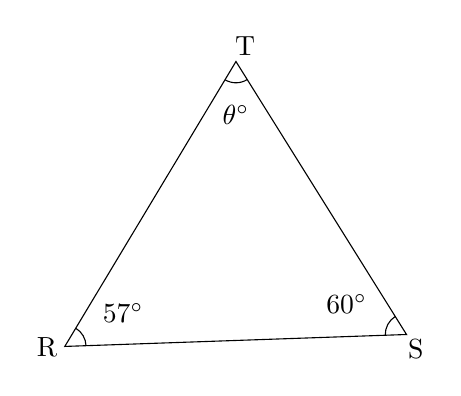
\begin{tikzpicture}[scale=0.9, baseline=(current bounding box.north)]
        \begin{scope}[rotate=2]
            \coordinate (A) at (0,0);
            \coordinate (B) at (4.825,0);
            \coordinate (C) at (intersection cs: first line={(A)--($(A)+(57:4cm)$)}, second line={(B)--($(B)+(180-60:4cm)$)});
            \draw (A) -- (B) -- (C) -- cycle;

            % Mark angles with arcs;
            \draw ($(A)!0.3cm!(B)$) arc [start angle=0, end angle=57, radius=0.3cm];
            \draw ($(B)!0.3cm!(C)$) arc [start angle=180-60, end angle=180, radius=0.3cm];
            \draw ($(C)!0.3cm!(A)$) arc [start angle=180+57, end angle=360-60, radius=0.3cm];

            % Label angles
            \node at ($(A)!-0.25cm!(B)$) {R};
            \node at ($(B)!-0.25cm!(C)$) {S};
            \node at ($(C)!-0.25cm!(A)$) {T};

            % Mark angles in degrees
            \coordinate (midBC) at ($(B)!0.5!(C)$);
            \node at ($(A)!0.95cm!(midBC)$) {$57^\circ$};

            \coordinate (midAC) at ($(A)!0.5!(C)$);
            \node at ($(B)!0.95cm!(midAC)$) {$60^\circ$};

            \coordinate (midAB) at ($(A)!0.5!(B)$);
            \node at ($(C)!0.75cm!(midAB)$) {$\theta^\circ$};

          \end{scope}
        \end{tikzpicture}
    \end{minipage}%
    \hfill
    \begin{minipage}{0.4\textwidth}
        \begin{align*}
        \text{$\theta^\circ$} &= 180^\circ - (\angle \text{\dotuline{~~~~~~~}} + \angle \text{\dotuline{~~~~~~~}}) \\
        &= 180^\circ - (\dotuline{~~~~~~~}^\circ + \dotuline{~~~~~~~}^\circ) \\
        &= 180^\circ - \dotuline{~~~~~~~}^\circ \\
        &= \dotuline{~~~~~~~}^\circ
        \end{align*}
    \end{minipage}

\vspace{1cm} \vfill\pagebreak ~ \newline ~ \newline    \begin{minipage}{0.55\textwidth}
    \refstepcounter{minipagecount}
    \noindent{(\theminipagecount)}\quad
    \begin{tikzpicture}[scale=0.9, baseline=(current bounding box.north)]
        \begin{scope}[rotate=198]
            \coordinate (A) at (0,0);
            \coordinate (B) at (5.025,0);
            \coordinate (C) at (intersection cs: first line={(A)--($(A)+(40:4cm)$)}, second line={(B)--($(B)+(180-69:4cm)$)});
            \draw (A) -- (B) -- (C) -- cycle;

            % Mark angles with arcs;
            \draw ($(A)!0.3cm!(B)$) arc [start angle=0, end angle=40, radius=0.3cm];
            \draw ($(B)!0.3cm!(C)$) arc [start angle=180-69, end angle=180, radius=0.3cm];
            \draw ($(C)!0.3cm!(A)$) arc [start angle=180+40, end angle=360-69, radius=0.3cm];

            % Label angles
            \node at ($(A)!-0.25cm!(B)$) {Z};
            \node at ($(B)!-0.25cm!(C)$) {X};
            \node at ($(C)!-0.25cm!(A)$) {Y};

            % Mark angles in degrees
            \coordinate (midBC) at ($(B)!0.5!(C)$);
            \node at ($(A)!0.95cm!(midBC)$) {$40^\circ$};

            \coordinate (midAC) at ($(A)!0.5!(C)$);
            \node at ($(B)!0.95cm!(midAC)$) {$69^\circ$};

            \coordinate (midAB) at ($(A)!0.5!(B)$);
            \node at ($(C)!0.75cm!(midAB)$) {$\theta^\circ$};

          \end{scope}
        \end{tikzpicture}
    \end{minipage}%
    \hfill
    \begin{minipage}{0.4\textwidth}
        \begin{align*}
        \text{$\theta^\circ$} &= 180^\circ - (\angle \text{\dotuline{~~~~~~~}} + \angle \text{\dotuline{~~~~~~~}}) \\
        &= 180^\circ - (\dotuline{~~~~~~~}^\circ + \dotuline{~~~~~~~}^\circ) \\
        &= 180^\circ - \dotuline{~~~~~~~}^\circ \\
        &= \dotuline{~~~~~~~}^\circ
        \end{align*}
    \end{minipage}

\vspace{1cm} \vfill    \begin{minipage}{0.55\textwidth}
    \refstepcounter{minipagecount}
    \noindent{(\theminipagecount)}\quad
    \begin{tikzpicture}[scale=0.9, baseline=(current bounding box.north)]
        \begin{scope}[rotate=294]
            \coordinate (A) at (0,0);
            \coordinate (B) at (5.15,0);
            \coordinate (C) at (intersection cs: first line={(A)--($(A)+(44:4cm)$)}, second line={(B)--($(B)+(180-60:4cm)$)});
            \draw (A) -- (B) -- (C) -- cycle;

            % Mark angles with arcs;
            \draw ($(A)!0.3cm!(B)$) arc [start angle=0, end angle=44, radius=0.3cm];
            \draw ($(B)!0.3cm!(C)$) arc [start angle=180-60, end angle=180, radius=0.3cm];
            \draw ($(C)!0.3cm!(A)$) arc [start angle=180+44, end angle=360-60, radius=0.3cm];

            % Label angles
            \node at ($(A)!-0.25cm!(B)$) {A};
            \node at ($(B)!-0.25cm!(C)$) {C};
            \node at ($(C)!-0.25cm!(A)$) {B};

            % Mark angles in degrees
            \coordinate (midBC) at ($(B)!0.5!(C)$);
            \node at ($(A)!0.95cm!(midBC)$) {$44^\circ$};

            \coordinate (midAC) at ($(A)!0.5!(C)$);
            \node at ($(B)!0.95cm!(midAC)$) {$60^\circ$};

            \coordinate (midAB) at ($(A)!0.5!(B)$);
            \node at ($(C)!0.75cm!(midAB)$) {$\theta^\circ$};

          \end{scope}
        \end{tikzpicture}
    \end{minipage}%
    \hfill
    \begin{minipage}{0.4\textwidth}
        \begin{align*}
        \text{$\theta^\circ$} &= 180^\circ - (\angle \text{\dotuline{~~~~~~~}} + \angle \text{\dotuline{~~~~~~~}}) \\
        &= 180^\circ - (\dotuline{~~~~~~~}^\circ + \dotuline{~~~~~~~}^\circ) \\
        &= 180^\circ - \dotuline{~~~~~~~}^\circ \\
        &= \dotuline{~~~~~~~}^\circ
        \end{align*}
    \end{minipage}

\vspace{1cm} \vfill    \begin{minipage}{0.55\textwidth}
    \refstepcounter{minipagecount}
    \noindent{(\theminipagecount)}\quad
    \begin{tikzpicture}[scale=0.9, baseline=(current bounding box.north)]
        \begin{scope}[rotate=108]
            \coordinate (A) at (0,0);
            \coordinate (B) at (5.025,0);
            \coordinate (C) at (intersection cs: first line={(A)--($(A)+(46:4cm)$)}, second line={(B)--($(B)+(180-63:4cm)$)});
            \draw (A) -- (B) -- (C) -- cycle;

            % Mark angles with arcs;
            \draw ($(A)!0.3cm!(B)$) arc [start angle=0, end angle=46, radius=0.3cm];
            \draw ($(B)!0.3cm!(C)$) arc [start angle=180-63, end angle=180, radius=0.3cm];
            \draw ($(C)!0.3cm!(A)$) arc [start angle=180+46, end angle=360-63, radius=0.3cm];

            % Label angles
            \node at ($(A)!-0.25cm!(B)$) {T};
            \node at ($(B)!-0.25cm!(C)$) {S};
            \node at ($(C)!-0.25cm!(A)$) {R};

            % Mark angles in degrees
            \coordinate (midBC) at ($(B)!0.5!(C)$);
            \node at ($(A)!0.95cm!(midBC)$) {$46^\circ$};

            \coordinate (midAC) at ($(A)!0.5!(C)$);
            \node at ($(B)!0.95cm!(midAC)$) {$63^\circ$};

            \coordinate (midAB) at ($(A)!0.5!(B)$);
            \node at ($(C)!0.75cm!(midAB)$) {$\theta^\circ$};

          \end{scope}
        \end{tikzpicture}
    \end{minipage}%
    \hfill
    \begin{minipage}{0.4\textwidth}
        \begin{align*}
        \text{$\theta^\circ$} &= 180^\circ - (\angle \text{\dotuline{~~~~~~~}} + \angle \text{\dotuline{~~~~~~~}}) \\
        &= 180^\circ - (\dotuline{~~~~~~~}^\circ + \dotuline{~~~~~~~}^\circ) \\
        &= 180^\circ - \dotuline{~~~~~~~}^\circ \\
        &= \dotuline{~~~~~~~}^\circ
        \end{align*}
    \end{minipage}

\vspace{1cm} \vfill    \begin{minipage}{0.55\textwidth}
    \refstepcounter{minipagecount}
    \noindent{(\theminipagecount)}\quad
    \begin{tikzpicture}[scale=0.9, baseline=(current bounding box.north)]
        \begin{scope}[rotate=33]
            \coordinate (A) at (0,0);
            \coordinate (B) at (4.925,0);
            \coordinate (C) at (intersection cs: first line={(A)--($(A)+(54:4cm)$)}, second line={(B)--($(B)+(180-59:4cm)$)});
            \draw (A) -- (B) -- (C) -- cycle;

            % Mark angles with arcs;
            \draw ($(A)!0.3cm!(B)$) arc [start angle=0, end angle=54, radius=0.3cm];
            \draw ($(B)!0.3cm!(C)$) arc [start angle=180-59, end angle=180, radius=0.3cm];
            \draw ($(C)!0.3cm!(A)$) arc [start angle=180+54, end angle=360-59, radius=0.3cm];

            % Label angles
            \node at ($(A)!-0.25cm!(B)$) {Z};
            \node at ($(B)!-0.25cm!(C)$) {Y};
            \node at ($(C)!-0.25cm!(A)$) {X};

            % Mark angles in degrees
            \coordinate (midBC) at ($(B)!0.5!(C)$);
            \node at ($(A)!0.95cm!(midBC)$) {$54^\circ$};

            \coordinate (midAC) at ($(A)!0.5!(C)$);
            \node at ($(B)!0.95cm!(midAC)$) {$59^\circ$};

            \coordinate (midAB) at ($(A)!0.5!(B)$);
            \node at ($(C)!0.75cm!(midAB)$) {$\theta^\circ$};

          \end{scope}
        \end{tikzpicture}
    \end{minipage}%
    \hfill
    \begin{minipage}{0.4\textwidth}
        \begin{align*}
        \text{$\theta^\circ$} &= 180^\circ - (\angle \text{\dotuline{~~~~~~~}} + \angle \text{\dotuline{~~~~~~~}}) \\
        &= 180^\circ - (\dotuline{~~~~~~~}^\circ + \dotuline{~~~~~~~}^\circ) \\
        &= 180^\circ - \dotuline{~~~~~~~}^\circ \\
        &= \dotuline{~~~~~~~}^\circ
        \end{align*}
    \end{minipage}

\vspace{1cm} \vfill\pagebreak ~ \newline ~ \newline    \begin{minipage}{0.55\textwidth}
    \refstepcounter{minipagecount}
    \noindent{(\theminipagecount)}\quad
    \begin{tikzpicture}[scale=0.9, baseline=(current bounding box.north)]
        \begin{scope}[rotate=352]
            \coordinate (A) at (0,0);
            \coordinate (B) at (4.85,0);
            \coordinate (C) at (intersection cs: first line={(A)--($(A)+(72:4cm)$)}, second line={(B)--($(B)+(180-44:4cm)$)});
            \draw (A) -- (B) -- (C) -- cycle;

            % Mark angles with arcs;
            \draw ($(A)!0.3cm!(B)$) arc [start angle=0, end angle=72, radius=0.3cm];
            \draw ($(B)!0.3cm!(C)$) arc [start angle=180-44, end angle=180, radius=0.3cm];
            \draw ($(C)!0.3cm!(A)$) arc [start angle=180+72, end angle=360-44, radius=0.3cm];

            % Label angles
            \node at ($(A)!-0.25cm!(B)$) {A};
            \node at ($(B)!-0.25cm!(C)$) {C};
            \node at ($(C)!-0.25cm!(A)$) {B};

            % Mark angles in degrees
            \coordinate (midBC) at ($(B)!0.5!(C)$);
            \node at ($(A)!0.95cm!(midBC)$) {$72^\circ$};

            \coordinate (midAC) at ($(A)!0.5!(C)$);
            \node at ($(B)!0.95cm!(midAC)$) {$44^\circ$};

            \coordinate (midAB) at ($(A)!0.5!(B)$);
            \node at ($(C)!0.75cm!(midAB)$) {$\theta^\circ$};

          \end{scope}
        \end{tikzpicture}
    \end{minipage}%
    \hfill
    \begin{minipage}{0.4\textwidth}
        \begin{align*}
        \text{$\theta^\circ$} &= 180^\circ - (\angle \text{\dotuline{~~~~~~~}} + \angle \text{\dotuline{~~~~~~~}}) \\
        &= 180^\circ - (\dotuline{~~~~~~~}^\circ + \dotuline{~~~~~~~}^\circ) \\
        &= 180^\circ - \dotuline{~~~~~~~}^\circ \\
        &= \dotuline{~~~~~~~}^\circ
        \end{align*}
    \end{minipage}

\vspace{1cm} \vfill    \begin{minipage}{0.55\textwidth}
    \refstepcounter{minipagecount}
    \noindent{(\theminipagecount)}\quad
    \begin{tikzpicture}[scale=0.9, baseline=(current bounding box.north)]
        \begin{scope}[rotate=126]
            \coordinate (A) at (0,0);
            \coordinate (B) at (5.175,0);
            \coordinate (C) at (intersection cs: first line={(A)--($(A)+(48:4cm)$)}, second line={(B)--($(B)+(180-55:4cm)$)});
            \draw (A) -- (B) -- (C) -- cycle;

            % Mark angles with arcs;
            \draw ($(A)!0.3cm!(B)$) arc [start angle=0, end angle=48, radius=0.3cm];
            \draw ($(B)!0.3cm!(C)$) arc [start angle=180-55, end angle=180, radius=0.3cm];
            \draw ($(C)!0.3cm!(A)$) arc [start angle=180+48, end angle=360-55, radius=0.3cm];

            % Label angles
            \node at ($(A)!-0.25cm!(B)$) {A};
            \node at ($(B)!-0.25cm!(C)$) {C};
            \node at ($(C)!-0.25cm!(A)$) {B};

            % Mark angles in degrees
            \coordinate (midBC) at ($(B)!0.5!(C)$);
            \node at ($(A)!0.95cm!(midBC)$) {$48^\circ$};

            \coordinate (midAC) at ($(A)!0.5!(C)$);
            \node at ($(B)!0.95cm!(midAC)$) {$55^\circ$};

            \coordinate (midAB) at ($(A)!0.5!(B)$);
            \node at ($(C)!0.75cm!(midAB)$) {$\theta^\circ$};

          \end{scope}
        \end{tikzpicture}
    \end{minipage}%
    \hfill
    \begin{minipage}{0.4\textwidth}
        \begin{align*}
        \text{$\theta^\circ$} &= 180^\circ - (\angle \text{\dotuline{~~~~~~~}} + \angle \text{\dotuline{~~~~~~~}}) \\
        &= 180^\circ - (\dotuline{~~~~~~~}^\circ + \dotuline{~~~~~~~}^\circ) \\
        &= 180^\circ - \dotuline{~~~~~~~}^\circ \\
        &= \dotuline{~~~~~~~}^\circ
        \end{align*}
    \end{minipage}

\vspace{1cm} \vfill    \begin{minipage}{0.55\textwidth}
    \refstepcounter{minipagecount}
    \noindent{(\theminipagecount)}\quad
    \begin{tikzpicture}[scale=0.9, baseline=(current bounding box.north)]
        \begin{scope}[rotate=43]
            \coordinate (A) at (0,0);
            \coordinate (B) at (4.675,0);
            \coordinate (C) at (intersection cs: first line={(A)--($(A)+(53:4cm)$)}, second line={(B)--($(B)+(180-70:4cm)$)});
            \draw (A) -- (B) -- (C) -- cycle;

            % Mark angles with arcs;
            \draw ($(A)!0.3cm!(B)$) arc [start angle=0, end angle=53, radius=0.3cm];
            \draw ($(B)!0.3cm!(C)$) arc [start angle=180-70, end angle=180, radius=0.3cm];
            \draw ($(C)!0.3cm!(A)$) arc [start angle=180+53, end angle=360-70, radius=0.3cm];

            % Label angles
            \node at ($(A)!-0.25cm!(B)$) {S};
            \node at ($(B)!-0.25cm!(C)$) {T};
            \node at ($(C)!-0.25cm!(A)$) {R};

            % Mark angles in degrees
            \coordinate (midBC) at ($(B)!0.5!(C)$);
            \node at ($(A)!0.95cm!(midBC)$) {$53^\circ$};

            \coordinate (midAC) at ($(A)!0.5!(C)$);
            \node at ($(B)!0.95cm!(midAC)$) {$70^\circ$};

            \coordinate (midAB) at ($(A)!0.5!(B)$);
            \node at ($(C)!0.75cm!(midAB)$) {$\theta^\circ$};

          \end{scope}
        \end{tikzpicture}
    \end{minipage}%
    \hfill
    \begin{minipage}{0.4\textwidth}
        \begin{align*}
        \text{$\theta^\circ$} &= 180^\circ - (\angle \text{\dotuline{~~~~~~~}} + \angle \text{\dotuline{~~~~~~~}}) \\
        &= 180^\circ - (\dotuline{~~~~~~~}^\circ + \dotuline{~~~~~~~}^\circ) \\
        &= 180^\circ - \dotuline{~~~~~~~}^\circ \\
        &= \dotuline{~~~~~~~}^\circ
        \end{align*}
    \end{minipage}

\vspace{1cm} \vfill    \begin{minipage}{0.55\textwidth}
    \refstepcounter{minipagecount}
    \noindent{(\theminipagecount)}\quad
    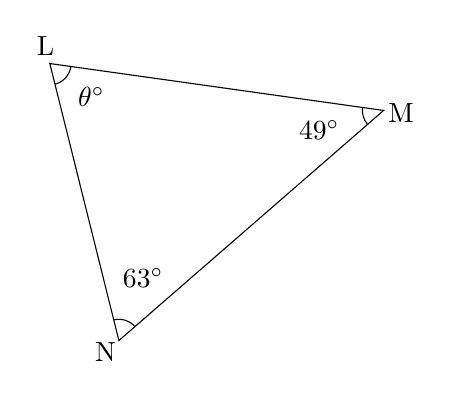
\begin{tikzpicture}[scale=0.9, baseline=(current bounding box.north)]
        \begin{scope}[rotate=41]
            \coordinate (A) at (0,0);
            \coordinate (B) at (4.95,0);
            \coordinate (C) at (intersection cs: first line={(A)--($(A)+(63:4cm)$)}, second line={(B)--($(B)+(180-49:4cm)$)});
            \draw (A) -- (B) -- (C) -- cycle;

            % Mark angles with arcs;
            \draw ($(A)!0.3cm!(B)$) arc [start angle=0, end angle=63, radius=0.3cm];
            \draw ($(B)!0.3cm!(C)$) arc [start angle=180-49, end angle=180, radius=0.3cm];
            \draw ($(C)!0.3cm!(A)$) arc [start angle=180+63, end angle=360-49, radius=0.3cm];

            % Label angles
            \node at ($(A)!-0.25cm!(B)$) {N};
            \node at ($(B)!-0.25cm!(C)$) {M};
            \node at ($(C)!-0.25cm!(A)$) {L};

            % Mark angles in degrees
            \coordinate (midBC) at ($(B)!0.5!(C)$);
            \node at ($(A)!0.95cm!(midBC)$) {$63^\circ$};

            \coordinate (midAC) at ($(A)!0.5!(C)$);
            \node at ($(B)!0.95cm!(midAC)$) {$49^\circ$};

            \coordinate (midAB) at ($(A)!0.5!(B)$);
            \node at ($(C)!0.75cm!(midAB)$) {$\theta^\circ$};

          \end{scope}
        \end{tikzpicture}
    \end{minipage}%
    \hfill
    \begin{minipage}{0.4\textwidth}
        \begin{align*}
        \text{$\theta^\circ$} &= 180^\circ - (\angle \text{\dotuline{~~~~~~~}} + \angle \text{\dotuline{~~~~~~~}}) \\
        &= 180^\circ - (\dotuline{~~~~~~~}^\circ + \dotuline{~~~~~~~}^\circ) \\
        &= 180^\circ - \dotuline{~~~~~~~}^\circ \\
        &= \dotuline{~~~~~~~}^\circ
        \end{align*}
    \end{minipage}

\vspace{1cm} \vfill\pagebreak ~ \newline ~ \newline    \begin{minipage}{0.55\textwidth}
    \refstepcounter{minipagecount}
    \noindent{(\theminipagecount)}\quad
    \begin{tikzpicture}[scale=0.9, baseline=(current bounding box.north)]
        \begin{scope}[rotate=112]
            \coordinate (A) at (0,0);
            \coordinate (B) at (4.125,0);
            \coordinate (C) at (intersection cs: first line={(A)--($(A)+(75:4cm)$)}, second line={(B)--($(B)+(180-70:4cm)$)});
            \draw (A) -- (B) -- (C) -- cycle;

            % Mark angles with arcs;
            \draw ($(A)!0.3cm!(B)$) arc [start angle=0, end angle=75, radius=0.3cm];
            \draw ($(B)!0.3cm!(C)$) arc [start angle=180-70, end angle=180, radius=0.3cm];
            \draw ($(C)!0.3cm!(A)$) arc [start angle=180+75, end angle=360-70, radius=0.3cm];

            % Label angles
            \node at ($(A)!-0.25cm!(B)$) {X};
            \node at ($(B)!-0.25cm!(C)$) {Y};
            \node at ($(C)!-0.25cm!(A)$) {Z};

            % Mark angles in degrees
            \coordinate (midBC) at ($(B)!0.5!(C)$);
            \node at ($(A)!0.95cm!(midBC)$) {$75^\circ$};

            \coordinate (midAC) at ($(A)!0.5!(C)$);
            \node at ($(B)!0.95cm!(midAC)$) {$70^\circ$};

            \coordinate (midAB) at ($(A)!0.5!(B)$);
            \node at ($(C)!0.75cm!(midAB)$) {$\theta^\circ$};

          \end{scope}
        \end{tikzpicture}
    \end{minipage}%
    \hfill
    \begin{minipage}{0.4\textwidth}
        \begin{align*}
        \text{$\theta^\circ$} &= 180^\circ - (\angle \text{\dotuline{~~~~~~~}} + \angle \text{\dotuline{~~~~~~~}}) \\
        &= 180^\circ - (\dotuline{~~~~~~~}^\circ + \dotuline{~~~~~~~}^\circ) \\
        &= 180^\circ - \dotuline{~~~~~~~}^\circ \\
        &= \dotuline{~~~~~~~}^\circ
        \end{align*}
    \end{minipage}

\vspace{1cm} \vfill    \begin{minipage}{0.55\textwidth}
    \refstepcounter{minipagecount}
    \noindent{(\theminipagecount)}\quad
    \begin{tikzpicture}[scale=0.9, baseline=(current bounding box.north)]
        \begin{scope}[rotate=248]
            \coordinate (A) at (0,0);
            \coordinate (B) at (4.775,0);
            \coordinate (C) at (intersection cs: first line={(A)--($(A)+(45:4cm)$)}, second line={(B)--($(B)+(180-74:4cm)$)});
            \draw (A) -- (B) -- (C) -- cycle;

            % Mark angles with arcs;
            \draw ($(A)!0.3cm!(B)$) arc [start angle=0, end angle=45, radius=0.3cm];
            \draw ($(B)!0.3cm!(C)$) arc [start angle=180-74, end angle=180, radius=0.3cm];
            \draw ($(C)!0.3cm!(A)$) arc [start angle=180+45, end angle=360-74, radius=0.3cm];

            % Label angles
            \node at ($(A)!-0.25cm!(B)$) {C};
            \node at ($(B)!-0.25cm!(C)$) {A};
            \node at ($(C)!-0.25cm!(A)$) {B};

            % Mark angles in degrees
            \coordinate (midBC) at ($(B)!0.5!(C)$);
            \node at ($(A)!0.95cm!(midBC)$) {$45^\circ$};

            \coordinate (midAC) at ($(A)!0.5!(C)$);
            \node at ($(B)!0.95cm!(midAC)$) {$74^\circ$};

            \coordinate (midAB) at ($(A)!0.5!(B)$);
            \node at ($(C)!0.75cm!(midAB)$) {$\theta^\circ$};

          \end{scope}
        \end{tikzpicture}
    \end{minipage}%
    \hfill
    \begin{minipage}{0.4\textwidth}
        \begin{align*}
        \text{$\theta^\circ$} &= 180^\circ - (\angle \text{\dotuline{~~~~~~~}} + \angle \text{\dotuline{~~~~~~~}}) \\
        &= 180^\circ - (\dotuline{~~~~~~~}^\circ + \dotuline{~~~~~~~}^\circ) \\
        &= 180^\circ - \dotuline{~~~~~~~}^\circ \\
        &= \dotuline{~~~~~~~}^\circ
        \end{align*}
    \end{minipage}

\vspace{1cm} \vfill    \begin{minipage}{0.55\textwidth}
    \refstepcounter{minipagecount}
    \noindent{(\theminipagecount)}\quad
    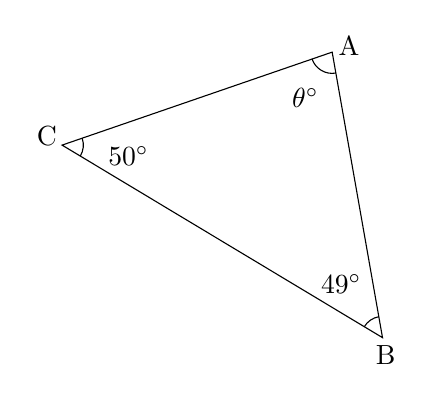
\begin{tikzpicture}[scale=0.9, baseline=(current bounding box.north)]
        \begin{scope}[rotate=329]
            \coordinate (A) at (0,0);
            \coordinate (B) at (5.275,0);
            \coordinate (C) at (intersection cs: first line={(A)--($(A)+(50:4cm)$)}, second line={(B)--($(B)+(180-49:4cm)$)});
            \draw (A) -- (B) -- (C) -- cycle;

            % Mark angles with arcs;
            \draw ($(A)!0.3cm!(B)$) arc [start angle=0, end angle=50, radius=0.3cm];
            \draw ($(B)!0.3cm!(C)$) arc [start angle=180-49, end angle=180, radius=0.3cm];
            \draw ($(C)!0.3cm!(A)$) arc [start angle=180+50, end angle=360-49, radius=0.3cm];

            % Label angles
            \node at ($(A)!-0.25cm!(B)$) {C};
            \node at ($(B)!-0.25cm!(C)$) {B};
            \node at ($(C)!-0.25cm!(A)$) {A};

            % Mark angles in degrees
            \coordinate (midBC) at ($(B)!0.5!(C)$);
            \node at ($(A)!0.95cm!(midBC)$) {$50^\circ$};

            \coordinate (midAC) at ($(A)!0.5!(C)$);
            \node at ($(B)!0.95cm!(midAC)$) {$49^\circ$};

            \coordinate (midAB) at ($(A)!0.5!(B)$);
            \node at ($(C)!0.75cm!(midAB)$) {$\theta^\circ$};

          \end{scope}
        \end{tikzpicture}
    \end{minipage}%
    \hfill
    \begin{minipage}{0.4\textwidth}
        \begin{align*}
        \text{$\theta^\circ$} &= 180^\circ - (\angle \text{\dotuline{~~~~~~~}} + \angle \text{\dotuline{~~~~~~~}}) \\
        &= 180^\circ - (\dotuline{~~~~~~~}^\circ + \dotuline{~~~~~~~}^\circ) \\
        &= 180^\circ - \dotuline{~~~~~~~}^\circ \\
        &= \dotuline{~~~~~~~}^\circ
        \end{align*}
    \end{minipage}

\vspace{1cm} \vfill    \begin{minipage}{0.55\textwidth}
    \refstepcounter{minipagecount}
    \noindent{(\theminipagecount)}\quad
    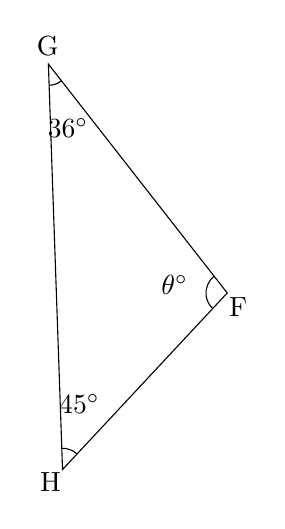
\begin{tikzpicture}[scale=0.9, baseline=(current bounding box.north)]
        \begin{scope}[rotate=272]
            \coordinate (A) at (0,0);
            \coordinate (B) at (5.725,0);
            \coordinate (C) at (intersection cs: first line={(A)--($(A)+(36:4cm)$)}, second line={(B)--($(B)+(180-45:4cm)$)});
            \draw (A) -- (B) -- (C) -- cycle;

            % Mark angles with arcs;
            \draw ($(A)!0.3cm!(B)$) arc [start angle=0, end angle=36, radius=0.3cm];
            \draw ($(B)!0.3cm!(C)$) arc [start angle=180-45, end angle=180, radius=0.3cm];
            \draw ($(C)!0.3cm!(A)$) arc [start angle=180+36, end angle=360-45, radius=0.3cm];

            % Label angles
            \node at ($(A)!-0.25cm!(B)$) {G};
            \node at ($(B)!-0.25cm!(C)$) {H};
            \node at ($(C)!-0.25cm!(A)$) {F};

            % Mark angles in degrees
            \coordinate (midBC) at ($(B)!0.5!(C)$);
            \node at ($(A)!0.95cm!(midBC)$) {$36^\circ$};

            \coordinate (midAC) at ($(A)!0.5!(C)$);
            \node at ($(B)!0.95cm!(midAC)$) {$45^\circ$};

            \coordinate (midAB) at ($(A)!0.5!(B)$);
            \node at ($(C)!0.75cm!(midAB)$) {$\theta^\circ$};

          \end{scope}
        \end{tikzpicture}
    \end{minipage}%
    \hfill
    \begin{minipage}{0.4\textwidth}
        \begin{align*}
        \text{$\theta^\circ$} &= 180^\circ - (\angle \text{\dotuline{~~~~~~~}} + \angle \text{\dotuline{~~~~~~~}}) \\
        &= 180^\circ - (\dotuline{~~~~~~~}^\circ + \dotuline{~~~~~~~}^\circ) \\
        &= 180^\circ - \dotuline{~~~~~~~}^\circ \\
        &= \dotuline{~~~~~~~}^\circ
        \end{align*}
    \end{minipage}

\vspace{1cm} \vfill\pagebreak ~ \newline ~ \newline    \begin{minipage}{0.55\textwidth}
    \refstepcounter{minipagecount}
    \noindent{(\theminipagecount)}\quad
    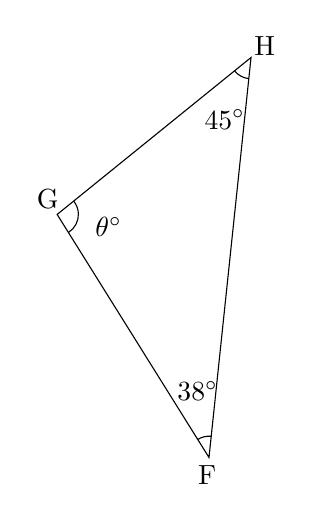
\begin{tikzpicture}[scale=0.9, baseline=(current bounding box.north)]
        \begin{scope}[rotate=84]
            \coordinate (A) at (0,0);
            \coordinate (B) at (5.675,0);
            \coordinate (C) at (intersection cs: first line={(A)--($(A)+(38:4cm)$)}, second line={(B)--($(B)+(180-45:4cm)$)});
            \draw (A) -- (B) -- (C) -- cycle;

            % Mark angles with arcs;
            \draw ($(A)!0.3cm!(B)$) arc [start angle=0, end angle=38, radius=0.3cm];
            \draw ($(B)!0.3cm!(C)$) arc [start angle=180-45, end angle=180, radius=0.3cm];
            \draw ($(C)!0.3cm!(A)$) arc [start angle=180+38, end angle=360-45, radius=0.3cm];

            % Label angles
            \node at ($(A)!-0.25cm!(B)$) {F};
            \node at ($(B)!-0.25cm!(C)$) {H};
            \node at ($(C)!-0.25cm!(A)$) {G};

            % Mark angles in degrees
            \coordinate (midBC) at ($(B)!0.5!(C)$);
            \node at ($(A)!0.95cm!(midBC)$) {$38^\circ$};

            \coordinate (midAC) at ($(A)!0.5!(C)$);
            \node at ($(B)!0.95cm!(midAC)$) {$45^\circ$};

            \coordinate (midAB) at ($(A)!0.5!(B)$);
            \node at ($(C)!0.75cm!(midAB)$) {$\theta^\circ$};

          \end{scope}
        \end{tikzpicture}
    \end{minipage}%
    \hfill
    \begin{minipage}{0.4\textwidth}
        \begin{align*}
        \text{$\theta^\circ$} &= 180^\circ - (\angle \text{\dotuline{~~~~~~~}} + \angle \text{\dotuline{~~~~~~~}}) \\
        &= 180^\circ - (\dotuline{~~~~~~~}^\circ + \dotuline{~~~~~~~}^\circ) \\
        &= 180^\circ - \dotuline{~~~~~~~}^\circ \\
        &= \dotuline{~~~~~~~}^\circ
        \end{align*}
    \end{minipage}

\vspace{1cm} \vfill    \begin{minipage}{0.55\textwidth}
    \refstepcounter{minipagecount}
    \noindent{(\theminipagecount)}\quad
    \begin{tikzpicture}[scale=0.9, baseline=(current bounding box.north)]
        \begin{scope}[rotate=330]
            \coordinate (A) at (0,0);
            \coordinate (B) at (4.525,0);
            \coordinate (C) at (intersection cs: first line={(A)--($(A)+(75:4cm)$)}, second line={(B)--($(B)+(180-54:4cm)$)});
            \draw (A) -- (B) -- (C) -- cycle;

            % Mark angles with arcs;
            \draw ($(A)!0.3cm!(B)$) arc [start angle=0, end angle=75, radius=0.3cm];
            \draw ($(B)!0.3cm!(C)$) arc [start angle=180-54, end angle=180, radius=0.3cm];
            \draw ($(C)!0.3cm!(A)$) arc [start angle=180+75, end angle=360-54, radius=0.3cm];

            % Label angles
            \node at ($(A)!-0.25cm!(B)$) {X};
            \node at ($(B)!-0.25cm!(C)$) {Y};
            \node at ($(C)!-0.25cm!(A)$) {Z};

            % Mark angles in degrees
            \coordinate (midBC) at ($(B)!0.5!(C)$);
            \node at ($(A)!0.95cm!(midBC)$) {$75^\circ$};

            \coordinate (midAC) at ($(A)!0.5!(C)$);
            \node at ($(B)!0.95cm!(midAC)$) {$54^\circ$};

            \coordinate (midAB) at ($(A)!0.5!(B)$);
            \node at ($(C)!0.75cm!(midAB)$) {$\theta^\circ$};

          \end{scope}
        \end{tikzpicture}
    \end{minipage}%
    \hfill
    \begin{minipage}{0.4\textwidth}
        \begin{align*}
        \text{$\theta^\circ$} &= 180^\circ - (\angle \text{\dotuline{~~~~~~~}} + \angle \text{\dotuline{~~~~~~~}}) \\
        &= 180^\circ - (\dotuline{~~~~~~~}^\circ + \dotuline{~~~~~~~}^\circ) \\
        &= 180^\circ - \dotuline{~~~~~~~}^\circ \\
        &= \dotuline{~~~~~~~}^\circ
        \end{align*}
    \end{minipage}

\vspace{1cm} \vfill    \begin{minipage}{0.55\textwidth}
    \refstepcounter{minipagecount}
    \noindent{(\theminipagecount)}\quad
    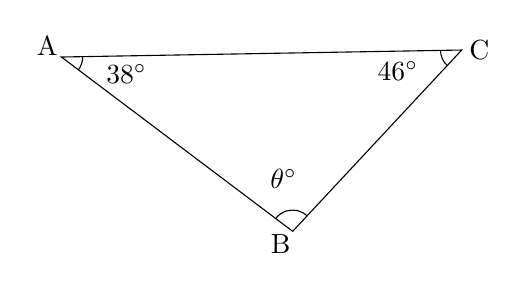
\begin{tikzpicture}[scale=0.9, baseline=(current bounding box.north)]
        \begin{scope}[rotate=181]
            \coordinate (A) at (0,0);
            \coordinate (B) at (5.65,0);
            \coordinate (C) at (intersection cs: first line={(A)--($(A)+(46:4cm)$)}, second line={(B)--($(B)+(180-38:4cm)$)});
            \draw (A) -- (B) -- (C) -- cycle;

            % Mark angles with arcs;
            \draw ($(A)!0.3cm!(B)$) arc [start angle=0, end angle=46, radius=0.3cm];
            \draw ($(B)!0.3cm!(C)$) arc [start angle=180-38, end angle=180, radius=0.3cm];
            \draw ($(C)!0.3cm!(A)$) arc [start angle=180+46, end angle=360-38, radius=0.3cm];

            % Label angles
            \node at ($(A)!-0.25cm!(B)$) {C};
            \node at ($(B)!-0.25cm!(C)$) {A};
            \node at ($(C)!-0.25cm!(A)$) {B};

            % Mark angles in degrees
            \coordinate (midBC) at ($(B)!0.5!(C)$);
            \node at ($(A)!0.95cm!(midBC)$) {$46^\circ$};

            \coordinate (midAC) at ($(A)!0.5!(C)$);
            \node at ($(B)!0.95cm!(midAC)$) {$38^\circ$};

            \coordinate (midAB) at ($(A)!0.5!(B)$);
            \node at ($(C)!0.75cm!(midAB)$) {$\theta^\circ$};

          \end{scope}
        \end{tikzpicture}
    \end{minipage}%
    \hfill
    \begin{minipage}{0.4\textwidth}
        \begin{align*}
        \text{$\theta^\circ$} &= 180^\circ - (\angle \text{\dotuline{~~~~~~~}} + \angle \text{\dotuline{~~~~~~~}}) \\
        &= 180^\circ - (\dotuline{~~~~~~~}^\circ + \dotuline{~~~~~~~}^\circ) \\
        &= 180^\circ - \dotuline{~~~~~~~}^\circ \\
        &= \dotuline{~~~~~~~}^\circ
        \end{align*}
    \end{minipage}

\vspace{1cm} \vfill    \begin{minipage}{0.55\textwidth}
    \refstepcounter{minipagecount}
    \noindent{(\theminipagecount)}\quad
    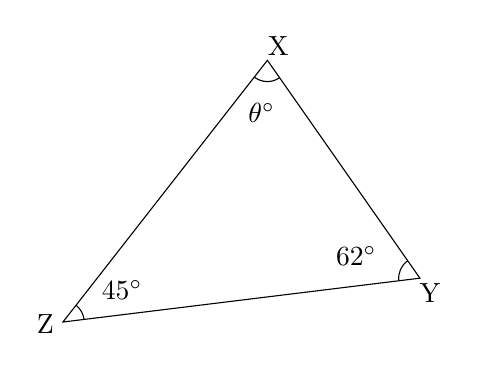
\begin{tikzpicture}[scale=0.9, baseline=(current bounding box.north)]
        \begin{scope}[rotate=7]
            \coordinate (A) at (0,0);
            \coordinate (B) at (5.075,0);
            \coordinate (C) at (intersection cs: first line={(A)--($(A)+(45:4cm)$)}, second line={(B)--($(B)+(180-62:4cm)$)});
            \draw (A) -- (B) -- (C) -- cycle;

            % Mark angles with arcs;
            \draw ($(A)!0.3cm!(B)$) arc [start angle=0, end angle=45, radius=0.3cm];
            \draw ($(B)!0.3cm!(C)$) arc [start angle=180-62, end angle=180, radius=0.3cm];
            \draw ($(C)!0.3cm!(A)$) arc [start angle=180+45, end angle=360-62, radius=0.3cm];

            % Label angles
            \node at ($(A)!-0.25cm!(B)$) {Z};
            \node at ($(B)!-0.25cm!(C)$) {Y};
            \node at ($(C)!-0.25cm!(A)$) {X};

            % Mark angles in degrees
            \coordinate (midBC) at ($(B)!0.5!(C)$);
            \node at ($(A)!0.95cm!(midBC)$) {$45^\circ$};

            \coordinate (midAC) at ($(A)!0.5!(C)$);
            \node at ($(B)!0.95cm!(midAC)$) {$62^\circ$};

            \coordinate (midAB) at ($(A)!0.5!(B)$);
            \node at ($(C)!0.75cm!(midAB)$) {$\theta^\circ$};

          \end{scope}
        \end{tikzpicture}
    \end{minipage}%
    \hfill
    \begin{minipage}{0.4\textwidth}
        \begin{align*}
        \text{$\theta^\circ$} &= 180^\circ - (\angle \text{\dotuline{~~~~~~~}} + \angle \text{\dotuline{~~~~~~~}}) \\
        &= 180^\circ - (\dotuline{~~~~~~~}^\circ + \dotuline{~~~~~~~}^\circ) \\
        &= 180^\circ - \dotuline{~~~~~~~}^\circ \\
        &= \dotuline{~~~~~~~}^\circ
        \end{align*}
    \end{minipage}

\vspace{1cm} \vfill

\end{document}
